\documentclass[border=0pt]{standalone}
\usepackage{tikz,amssymb,url,amsmath,amsthm,listings,algorithm,algpseudocode,enumerate, caption, xspace, float, verbatim,tabularx,mathtools,adjustbox,pgfplots}
\usetikzlibrary{fit}
\usetikzlibrary{positioning}
\usetikzlibrary{math}
\usetikzlibrary{shapes.misc}
\usetikzlibrary{backgrounds}
\def\bw{{\boldsymbol w}}
\def\bx{{\boldsymbol x}}
\def\balpha{{\boldsymbol \alpha}}
\pgfdeclarelayer{background}
\pgfsetlayers{background,main}
\tikzset{cross/.style={cross out, draw=black, minimum size=2*(#1-\pgflinewidth), inner sep=0pt, outer sep=0pt},cross/.default={1pt}}
\begin{document}
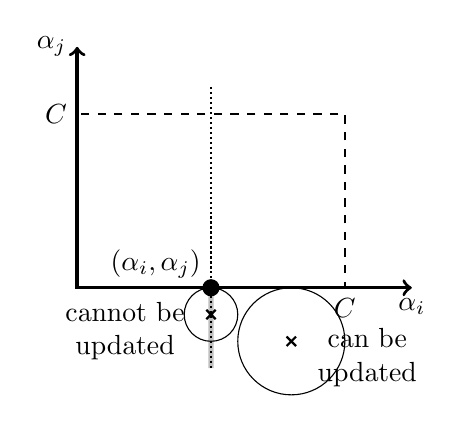
\begin{tikzpicture}[domain=-0.5:4,yscale=1.7,xscale=1.7,baseline,tight background]
	\tikzmath{\lx=0; \ly=0; \ux=2; \uy=1.3; \d=0.5;
	\dl=\lx-\d; \dr=\ux+\d; \da=\uy+\d; \db=\ly-\d;
	\dax=(\lx+\ux)/2; \day=\ly; \dbx=\ux; \dby=-\dax+\day+\dbx;
	\dda=0.8; \daax=\dax-\dda; \daay=\day-\dda; 
	\ddb=0.6; \dbax=\dbx+\ddb; \dbay=\dby+\ddb;
	\dab=0.2; \dabx=\dax; \daby=\uy+\dab; 
	\dbb=0.6; \dbbx=\dax; \dbby=\day-\dbb;
	\dac=0.2; \dacx=\dax-0.02; \dacy=\day; 
	\dbc=0.6; \dbcx=\dax-0.02; \dbcy=\day-\dbc;
	\dad=0.2; \dadx=\dax+0.02; \dady=\day; 
	\dbd=0.6; \dbdx=\dax+0.02; \dbdy=\day-\dbd;
	\ra=0.2 ;\cax=\dax; \cay=-\ra; 
	\rb=0.4; \cbx=\dax+0.6; \cby=-\rb;
	\caplx=0.35*\lx+0.65*\ux; \caply=\da;
	}
	\draw[-, dashed, thick] (\lx,\ly) -- (\ux,\ly) node[below]{$C$} -- (\ux,\uy) -- (\lx,\uy) node[left]{$C$} -- (\lx,\ly);
	\filldraw[black] (\dax,\day) node[above]{$(\alpha_i,\alpha_j)\qquad\quad\quad$} circle (1.7pt);
	\draw[<->, very thick] (\lx,\da) node[left]{$\alpha_j$} -- (\lx,\ly) -- (\dr,\ly) node[below]{$\alpha_i$};
	\draw[black] (\cax, \cay) node[left]{\begin{tabular}{c} \\ cannot be\\ updated\end{tabular}} circle (\ra);
	\draw (\cax, \cay) node[cross=2.5pt,thick]{};
	\draw[black] (\cbx, \cby) node[right]{\begin{tabular}{c} \\can be\\ updated\end{tabular}} circle (\rb);
	\draw (\cbx, \cby) node[cross=2.5pt,thick]{};
	\draw[-, densely dotted, thick] (\dabx, \daby) -- (\dbbx, \dbby);
	\begin{pgfonlayer}{background}
		\fill[lightgray] (\dacx,\dacy) to (\dbcx,\dbcy) to (\dbdx,\dbdy) to (\dadx,\dady) to (\dacx,\dady);
	\end{pgfonlayer}
	%\node at (\caplx, \caply){\;Without a Linear Constraint};
\end{tikzpicture}
\end{document}
